\documentclass[uplatex,b5j,8pt, twocolumn]{jsarticle}
\usepackage{etex}
\usepackage[dvipdfmx]{graphicx}
\usepackage{tikz} 
\usepackage{tikz-cd} 
\usepackage{tikz-qtree} 
\usepackage{ascmac,amscd,tabularx,begriff, amssymb,makeidx,dashrule,epic,eepic,wrapfig,latexsym,amsmath,listings,textcomp,mathrsfs,bigdelim,
multirow,accents,ulem}
\usepackage{pictexwd,dcpic}
\usepackage[LGR,T1]{fontenc}
\usepackage[OT2,OT1]{fontenc} \newcommand\cyr
{
\renewcommand\rmdefault{wncyr} \renewcommand\sfdefault{wncyss} \renewcommand\encodingdefault{OT2} \normalfont
\selectfont
}
\DeclareTextFontCommand{\textcyr}{\cyr} \def\cprime{\char"7E } \def\cdprime{\char"7F } \def\eoborotnoye{\char’013} \def\Eoborotnoye{\char’003}
\reserveinserts{28}
\newcommand{\textgreek}[1]{\begingroup\fontencoding{LGR}\selectfont#1\endgroup}
\makeatletter
\def\ruby#1#2{\leavevmode\vbox{%
\baselineskip\z@skip\lineskip.25ex
\ialign{##\crcr\rubyfont\hfill#2\hfill\crcr
\hfill#1\hfill\crcr}}}
\newcount\gpten % (global) power-of-ten -- tells which digit we are doing
\countdef\rtot2 % running total -- remainder so far
\countdef\LDscratch4 % scratch
\makeatother
\def\rubyfont{\tiny}
\renewcommand{\lstlistingname}{リスト}
\newcommand{\id}{\mathop{\mathrm{id}}\nolimits}
\usetikzlibrary{calc,decorations.pathmorphing,shapes}

\newcounter{sarrow}
\newcommand\xrsquigarrow[1]{%
\stepcounter{sarrow}%
\mathrel{\begin{tikzpicture}[baseline= {( $ (current bounding box.south) + (0,-0.5ex) $ )}]
\node[inner sep=.5ex] (\thesarrow) {$\scriptstyle #1$};
\path[draw,<-,decorate,
  decoration={zigzag,amplitude=0.7pt,segme11111111111111nt length=1.2mm,pre=lineto,pre length=4pt}] 
    (\thesarrow.south east) -- (\thesarrow.south west);
\end{tikzpicture}}%
}

\title{おんなのこLinux原稿 その1(2版)\\
{- アリストテレスとオブジェクト指向プログラミング -}}
\author{三番街侯爵(Marquis de Third)}
\date{
平成27年12月02日 
 }
\makeindex
\begin{document}
\maketitle

おんなのこLinux 原稿その1\copyright (2015) 横田 博史著\par

この著作の誤り, 誤植等で生じた損害に対して

著者は一切の責任を負いません.

\newpage
\setcounter{page}{1}

\section{はじめに}

ギリシャといえば今や国家の財政破綻や中近東の難民の大波ばかりが目立つ
状態ですが, ギリシャからさまざまな恩恵を我々は受けています. まず怪しいもの
にBLとGLの同性愛, そうでなく重要なものとしては神話, 詩や悲劇, 彫像や建築,
 そして哲学や論理学\footnote{論理学を発明・発展させた民族は他にインド人しか
いないのです. 中国戦国時代の墨家にも「墨子」\cite{墨子}から推論を含む論理学
があったことが伺えるのですが残念なことに途絶えています.}, 数学や天文学,
 そして医術等の科学全般といったものでしょうか.
\newline

BLでは古代ギリシャの都市国家テーバイ(\textgreek{J'hbai})の
「\textbf{神聖隊(\textgreek{>Ier'o L'oqos})}」\footnote{某アイドルグループ
とその所属事務所とは傾向等が似ていても違います.}を語らずにはいられません.
 この神聖隊は「\textbf{やおいのか硬いのか判らない}」のですが, 実際は
「\textbf{とてもやおく}」て「\textbf{とても硬い}」のです. まず
「\textbf{やおい}」ことについて語るなら, 神聖隊は恋人同士(勿論, 男同士です!)
150組, 300名で編成されていたそうです. 「\textbf{硬さ}」について語るなら,
 彼等は「\textbf{精鋭歩兵部隊}」だったのです.
\newline
 
 
\begin{wrapfigure}{l}{5cm}
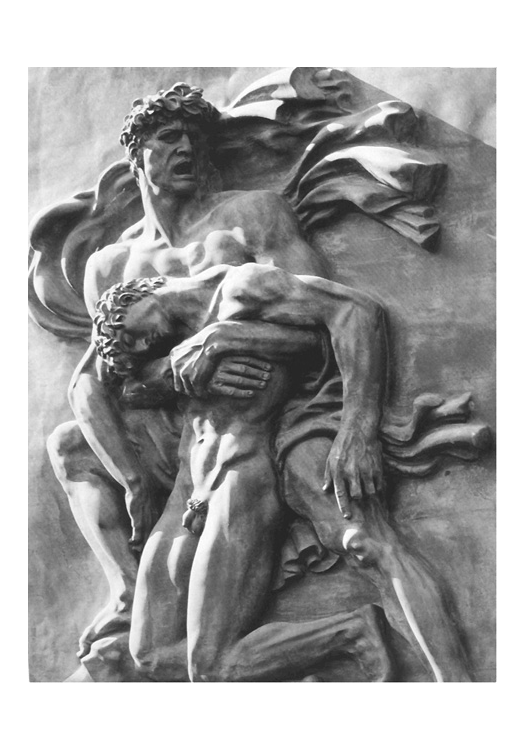
\includegraphics[width=5cm]{arno_breker_kameradschaft.pdf}
\caption{ブレーカー:戦友}
\label{fig:breker2}
\end{wrapfigure}

こういった部隊を編成した理由が, 恋人に無様な自分を見せたり危険な目に
合わせる訳にも行かないがために勇敢に戦うだろうとかで, 実際, テーバイ
をギリシャの覇権国家にする要因の一つになったと云います.
\newline

ところで神聖隊はマケドニア王国とギリシャの覇権を巡ってカロネイアの戦い
で王太子時代のアレクサンダー大王(\textgreek{>Al'exandros G'})率いる騎兵隊と
マケドニア式ファランクスの為に254名(丁度偶数!)が討死するという壊滅的打撃を
受けます. マケドニア王ピリッポス2世(\textgreek{F'ilippos B'})は彼等の亡骸を
見て涙したとのことですが, 戦いの半ば以降は図\ref{fig:breker2}の有様だった
ことでしょう. ちなみにこのレリーフはナチス時代の人気彫刻家ブレーカー
(Arno Breker)\footnote{ブレーカーの戦時中の手記が出版されていますが,
 その内容は非常にまともです.}のレリーフで, この味わいも現実の突撃隊の同性愛
を含む酒池肉林に変幻するというものでしょうか? たとえば図\ref{fig:rrevue}の
ように... 

\begin{figure}[htbp]
\begin{center}
\includegraphics[width=8cm]{DrittenReichsRevue.pdf}
\caption{第三帝国のレビューより\cite{関}}
\label{fig:rrevue}
\end{center}
\end{figure}

ここで茶化されているのは突撃隊幕僚長のレーム(R\"ohm)です. 彼はナチス
(NSDAP)の古参党員の一人で, その上, ヒトラー(Hitler)の古くからの友人でした.
 ところが彼は乱暴者, 生粋の男色家として著名で, 「\textbf{私のところにいる男
 たちは法律に反した特別な事に慣れねばならない}」と豪語し, 彼が在任中の突撃隊
で同性愛が横行したといいます. さらに彼は「国家社会主義」の「社会主義」に重点
を置いて「第二革命」を主張し, 突撃隊の国軍化を図ったことから国防軍に警戒され,
最終的に親衛隊によって所謂「長いナイフの夜」で粛清されてしまいます. この粛清
ではナチス左派が大量に粛清され, 粛清以降は同性愛は徹底的に禁じられることになり
ます\footnote{「ドイツ第三帝国」\cite{クラーザー}が文化的な側面にも言及があり
良い本です.また, ジョークについては「ヒトラー・ジョーク」\cite{関}が決定的で
しょう. この本からヴィスコンティ(Visconti)の「地獄に堕ちた勇者ども(The Damned)」
が連想される図\ref{fig:rrevue}を選びました.}
\newpage

\begin{wrapfigure}{l}{5cm}
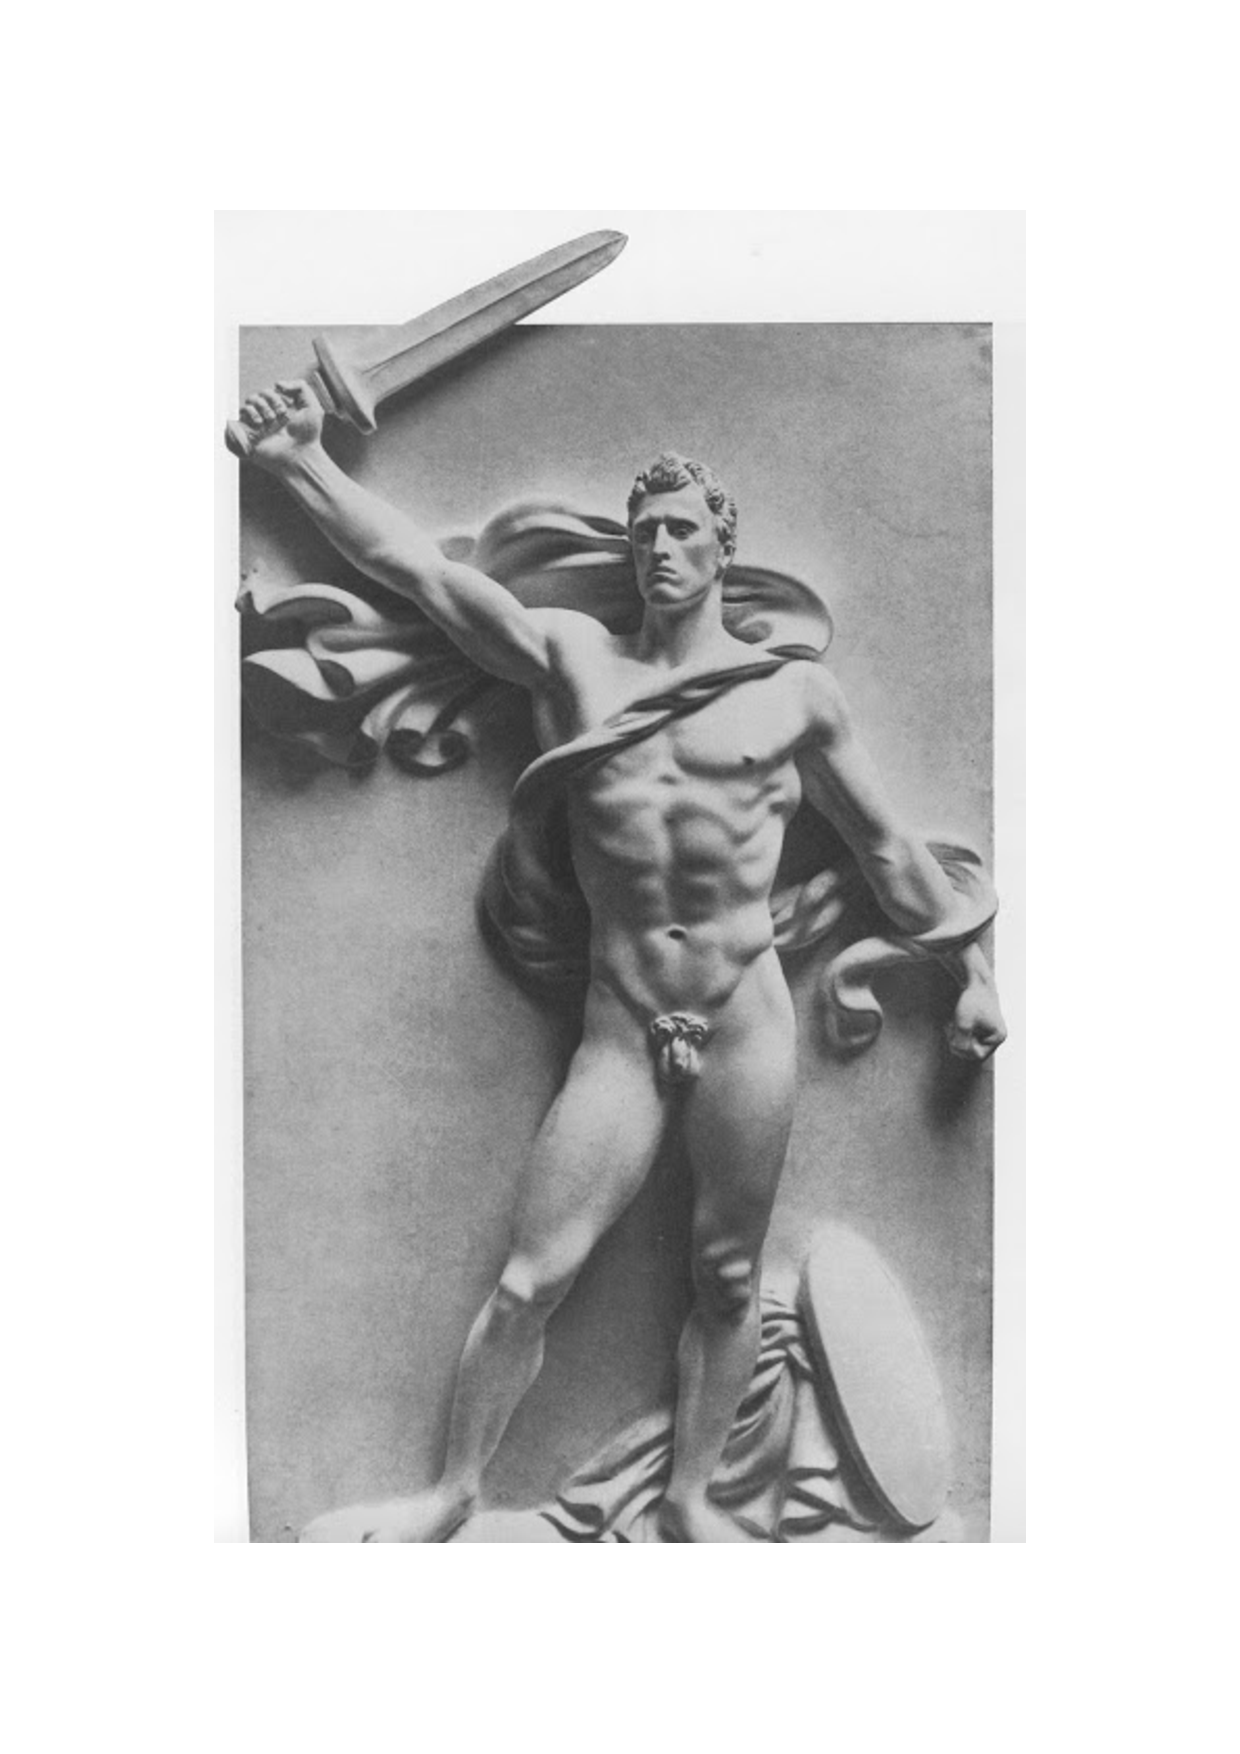
\includegraphics[width=6cm]{Breker2_relief.pdf}
\caption{ブレーカー:戦士の出発}
\label{fig:breker1}
\end{wrapfigure}

さてナチス公認芸術は図\ref{fig:breker2}のような英雄的なものに加え, 図\ref{fig:breker1}のように何だかよく判らないけどカッコエー代物
(裸体にマントがス・テ・キ$\heartsuit$)だとか, まあ随分と同性愛一歩手前の
際疾いものだったのです\footnote{女性絵画になると... ちなみに女性画の公認
巨匠ツィーグラー(Ziegler)は「\textbf{ドイツ恥毛の巨匠}」と呼ばれていたそう
です. それに苦言を呈する党員も居たそうですが「\textbf{兵士達は美しいものに
飢えているんだ!}」の一言で片付けられたとか.}. こういった代物でも, その胡散
臭さはさておき男の私でも「憧憬」を感じてしまうのです. 実際, こういった偉丈夫
に「\textbf{俺に付いて来い!}」と壁ドンされるとどうですか? 「\textbf{うほ!?}」
とならないにせよ「\textbf{面白い冒険が始まりそう..}」と思ってフラフラと
付いて行く男も多いのではないでしょうか? ただ, 古代ギリシャの同性愛は性的な
もの以上に「\textbf{若者は年長者の名声と知恵に憧れ, 年長者は若者の若さと
美に憧れる}」という至って素朴なものだったのではないかと私は思っています.
\newline

なお, ナチスはギリシャ文明を北方化したくて仕方なかったようです. 実際,
 歴史的にも北方からドーリア人(\textgreek{Dwrie'is})等の侵入がミケーネ
文明崩壊の原因の一つとされ, スパルタ(\textgreek{Spart'a})は先住民を征服して
とんでもない占領政策を続けているのでそう言いたくなるのも判らない訳でもあり
ません. これもゲーテ(G\"othe)が悲劇ファウスト(Faust)\cite{ゲーテ}で,
 本来の人形劇ファウストで絶世の美人の例でしかなかったヘレネー
(\textgreek{<El'enh})をヘレニズム文明そのものとし, それをドイツ・バロック的
なファウストと結婚させることで自らの古典主義を賛美したあたりからでしょか
\footnote{ヘレネー:「私はひどく遠くにいるような, そのくせ近くにいるような
気がします..」\cite{ゲーテ}第二部,第三幕}?  ゲーテはさておきその亜流連中に
とってはフランスがラテン文化の後継者なら, ドイツはより源流のギリシャ文明を
取るといった安易な民族主義が根幹にあったのかもしれません. なお, 野蛮な
ゲルマニアをそのまま受け入れるようになったのはロマン主義も後期に入ってから
のことです\footnote{当時のお隣のロシア帝国も同様で, 19世紀のチャイコフスキー({\cyr{Cha{\u i}kovski{\u i}}})のバレエは主に中世ドイツの宮廷やフランス的
な貴族の館の話ですが, 20世紀初頭のプロコフィエフ({\cyr{Prokof{\cprime}ev}})
やストラビンスキー({\cyr{Stravinski{\u i}}})になるとスキタイ人や古代ロシア人,
 でなければ民話といったあんばいです. では日本は? 政治的風潮で軍国主義を高貴と
讃え, 米英を卑しい商人の国と軽蔑したのが第一次世界大戦中のドイツ\cite{クラウス},
 日本ではそれを1930年代後半と20年近く遅れています.}.
\newline

ともあれナチスについて言えば, 19世紀末の夜郎自大的な民族主義にどっぷり染まり,
 ワーグナー(Wagner)のオペラの絢爛豪華さに感激した「\textbf{永遠の半端者}」,
 要するに2ちゃん用語の「\textbf{厨房共}」で, 「\textbf{聖なる愚か者}」の
Siegfriedを「\textbf{金髪の野蛮人}」に単純化し, それで彼等の青少年を染め上げ
た結果, のちにギリシャ文明の担い手になったドーリア人どころか西ローマ帝国を
崩壊させて暗黒時代を招来したヴァンダル族(Vandal)以上の想像を絶する惨禍を
招いてしまったのです. 19世紀初頭のドイツはヘルダーリン(H\"olderlin)によれば
「\textbf{人がいるが人間がいない!ドイツ人ほど支離滅裂な国民はいない.
 職人はいる, だが人間がいない. 思想家はいる,だが人間がいない. 牧師はいる,
 だが人間がいない.}」と嘆く有様で,  この状況はのちの哲学者ニーチェ(Nietzsche)
も同意し, 「ツァラトゥストラはこう言った」で 「\textbf{耳が肥大化した人間}」
等の戯画化で「\textbf{専門バカ}」や「\textbf{教養主義の俗物}」を茶化しているの
です(\cite{ツァラトゥストラ},救済)\footnote{ヘルダーリンのそれは
「ヒューペリオン」で失意の主人公がドイツに行ったときの感想です. ニーチェが
それを受けていることはその有様を「\textbf{戦場か屠殺場のように}」と
ヒューペリオンのものと同じ表現になっていることで判ります.}.
\newline

さて, ニーチェの著作「悲劇の誕生」\cite{悲劇の誕生}を読むと猛烈な古代
ギリシャへの憧れが見受けられます. この「悲劇の誕生」では
「ディオニューソス(\textgreek{Di'onusos})」的なるもの, すなわち, 情念と
「アポローン(\textgreek{>Ap'ollwn})」的なるもの, すなわち, 理念の対峙を主張
した論文で, 同時にワーグナーの楽劇をよいしょするものであったために
「\textbf{未来の文献学}」\footnote{ニーチェの本来の専門は文献学で,
 ワーグナーは自分の音楽のことを「\textbf{未来の音楽}」と呼んでいたことへの
当て付けです.}と皮肉られる結果になっています. その結びの一節に
「\textbf{美がこのように絶えず押し寄せてくる時...}」とありますが, 実に古代
ギリシャは偉大なのです. ところが我々日本人は残念なことに文明開化の時点で
目覚しく発展しつつあるプロシア=ドイツ帝国に目を奪われ, その結果, ドイツ好き
は沢山居ても, 西洋文明の源泉たるギリシャへの関心が斯くも少ないのが現状なの
です\footnote{文学では「潮騒」の三島由紀夫でしょうか.}.
\newline

そしてこの駄文の目標はギリシャ哲学と計算機科学を強引に結び付けようとする
分不相応な企てなのです. 時代を越えてファウストがヘレナに憧れ, 彼女と共に
あらんとするように私もそれを目指すのです.

\section{プラトンのイデア論}


さて主題の「\textbf{オブジェクト指向プログラミング(Object Oriented
 Programing)}」ですが, これはオブジェクトという概念を導入することで
プログラミングの生産性向上を図っているものと説明されます. 具体的にはクラス
というオブジェクトの雛形が用意され, その雛形を使ってプログラムが扱うデータ
に対応するインスタンスを生成して処理を行うこと. そして, クラスは属性や
メソッドをあらかじめ備えているので, そのインスタンスの処理でそれらが使える
こととクラスには親子関係に類似した階層構造があり, 属性やメソッドが継承と
呼ばれる手法で下位のクラスのインスタンスでも使えるという長所があることで
しょうか.
\newline


このオブジェクトがクラスから創られる有様を説明するためにプラトン
(\textgreek{Pl'atwn}, Plato)の「\textbf{イデア論(Theory of Forms)}」が引っ
張り出されることがあります. まず, プラトンのイデア論によれば我々が考察の
対象とする現世の「\textbf{個体(individual)}」に対しては
「\textbf{思惟によってのみ知られる世界}」, すなわち「\textbf{イデア界}」に
「\textbf{イデア(\textgreek{>id'ea}, idea)}」が存在し, 個体はそのイデアの
像であるというものです. だから貴方のそばに居る三毛猫の「\textbf{みけ}」には
対応する「\textbf{三毛猫のイデア}」が「\textbf{イデア界}」に存在し, その
イデアを現世に投影したものが貴方のそばに居る「\textbf{みけ}」であるという
主張です. なお, プラトンのイデアは思惟によってのみ知覚できることに加え,
 さらには「\textbf{永遠不滅}」といった超越的な性質を持っています. このこと
からイデアは現実にある対象を「\textbf{理想化したもの}」で, ちょうど
「\textbf{鋳型}」のような役割をしていると言えるでしょう. ただし, プラトン
はイデア界こそが真実の世界で, 現世はイデアが投影された「影の世界」, つまり
「\textbf{模倣物(\textgreek{e>ik'wn})}」の世界と見なしています(「洞窟の比喩」\cite{国家}).
\newline


ところでオブジェクトが計算機上のデータとして「\textbf{実体化}」する
ことを「\textbf{インスタンス化(instantiation)}」, それから
「\textbf{実体化したオブジェクト}」のことを
「\textbf{インスタンス(instance)}」と呼びますが, 
「\textbf{イデアの現世における実体化}」も英語では同じ
「\textbf{instantiation}」になります. と, このようにクラスとインスタンスの
関係はイデアと実物との関係に類似しています. さて, イデアを誰が実体化し,
 その実体化の理由は?という素朴な疑問になると途端にプラトンは歯切れが悪く
なります. まず誰がイデアを実体化させたのかと言えば,
 「\textbf{デーミウールゴス(\textgreek{dhmiourg'os})}」がイデアを模倣して
世界を創世し, その理由は貧欲な神「\textbf{エロース(\textgreek{>'Erws})}」が
イデアの美に憧れたからと述べていますが納得できるものではありません.
 また, イデアは美や善に関わるもので醜いものや悪にイデアは存在しないと
述べていますが, 「\textbf{何が美なのかをヒキガエルに聞いてみろ!}」と
ヴォルテール(Voltaire)ならずとも言いたくもなるでしょう.
\newline


このような「\textbf{機械仕掛けの神(Deus ex machina)}」\footnote{
古代ギリシャ悲劇で収拾がつかなくなった話を解決するためにいきなり舞台に神
を登場させること(たとえばソフォクレース(\textgreek{Sofokl'hs})の悲劇
「ピロクテーテース(\textgreek{Filokt'hths})」の終盤に現われるヘーラクレース
(\textgreek{<Hraklhs}))がありましたが, その都合の良さに対する皮肉です.}を
持ち出されても信じるしかないところは哲学というよりも宗教です. 実際, のちの
ヘレニズム文明では, プラトンのイデア論を基に超越的な
「\textbf{一者(\textgreek{to >'en}, to hen)}」とその一者からの流出による
世界の創造(流出説)を取り入れた「\textbf{新プラトン主義}」\footnote{
「新プラトン主義」とは後世の呼び名で, その信奉者達はプラトンの考えに合致
するものと思っていました.}, デーミウールゴスによる悪しき世界の創造, 本質的
に不死でありながら星辰の支配を受け, 肉体に囚われた人間, そして死後の
超越的な神への帰一を柱とする「\textbf{グノーシス主義(\textgreek{Gnwsis})}」
\footnote{中近東では未だに少数派としてちらほら残っているようです.}へと繋
がります.
\newline


\begin{wrapfigure}{l}{4cm}
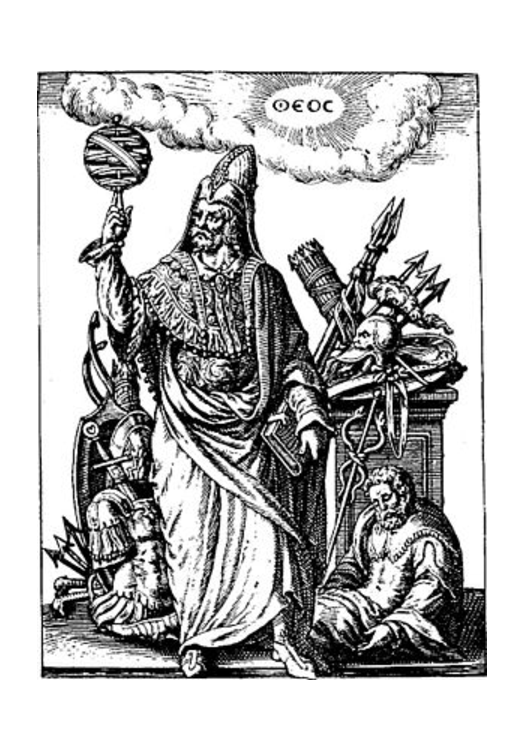
\includegraphics[width=4cm]{HermesTrismegistusCauc.pdf}
\caption{ヘルメス・トリスメギストス}
\label{fig:trismegistus}
\end{wrapfigure}

このグノーシス主義の文献に「 ヘルメス・トリスメギストス(三重に偉大なヘルメス,
 Hermes Trismegistus, \textgreek{<Erm\~es Trism'egistos})が記したとされた
\textbf{ヘルメス文書}」と呼ばれる一群の文書があります. ここでのヘルメスは
ギリシャ神話の神ヘルメスとエジプト神話の神トートがヘレニズム時代に融合した
もので, 錬金術では「\textbf{賢者の石}」\footnote{賢者の石は錬金術師が探し
求めた究極の霊薬で, 鉄などの非貴金属を貴金属の金に変え, 人間を不老不死に
するものです.}を実際に手にした人物\footnote{図\ref{fig:trismegistus}の
恰好の人物どこかで見たことありませんか? MITのSICP(Structure and
 Interpretation of Computer Programs)の扉絵の人物に似てますね.
 つまり$\lambda$ - 函数概念 - は計算機科学の「\textbf{賢者の石}」
で「\textbf{$A$ にして $\Omega$}」なのです!
Sanctus, sanctus, sanctus, dominus deus sabaoth.}とされています\cite{錬金術}.
そのヘルメス文書の一つの「ポイマンドレース(Poimandres)」\cite{柴田}によると
人間は元来, 神の子で美しい神の似姿として創られたとされます. その彼が高次で
純粋な天上界から下位の地上に向うことで星辰の支配を受け入れ\footnote{この宇宙観は太陽と惑星が同心同円状の配置された天動説に基くものです.}, 最後に地上にて
フュシス(\textgreek{f'usis}, 自然)内に写った自分の姿に恋することでフュシスと
愛欲に陥いり「\textbf{フュシスは愛する者を捕へ, 全身で抱きしめて互に交わった}」
その結果, 人間はフュシスに捕えられてしまったといいます. この伝説\footnote{
おおよそ宗教, あるいは宗教的な代物はその伝説を続々と生成するものです. 現在でも
カトリックでは列聖で伝説が生成され, 共産主義はその英雄を量産するといった有様
です. 伝説や聖人を量産するのを止めて博物館や図書館で安心して閲覧できるように
なった時点が宗教の死です.}が人間の本質が神の似姿のために不死であるものの
消滅する肉体に囚われ, その上, 星辰に支配された存在であるという二面性を持つ
ことへの説明になっています. この伝説にはオリエント諸国の占星術の影響と
イデア論を中核に哲学が宗教へと変じて行く様子が刻印されているとも言えるでしょう.
\newline

この世はデーミウールゴスが誤って創造したものだという厭世的な観点は新プラトン
主義はもちろんのこと, キリスト教徒の主流派からも反駁されます\footnote{全知
全能の神が半端なことをする筈がないという反論です.}. それどころか本質的に
黙示的な宗教であったキリスト教は新プラトン主義の影響により徐々に合理的な
宗教へと変貌します. この変化は教父と呼ばれる神学者達によるもので, 若い
時分にマニ教徒\footnote{マニ教はグノーシス主義の宗教の中では最も勢力を奮った
世界宗教でした. 近年, 日本でもマニ教の曼荼羅絵が発見されている程です.}でも
あった教父アウグスティヌス(Augustinus Hipponensis, Augustine of Hippo)に
よって新プラトン主義が初期のキリスト教の理論付けに用いられます. その際に
新プラトン主義のフィルターを介した形でアリストテレス(\textgreek{>Aristot'elhs},
Aristotle)の哲学も部分的に導入されます. キリスト教と古代の間には大きな断絶が
あるのも事実ですが, ヘレニズム文明の同心円的な宇宙観, 星辰信仰やイシス信仰
をマリア崇敬として引継ぐ等, ヘレニズム文明を引き継いでいる一面もあるのです.
\newline

ここで本題に話を戻すと, プラトンのイデア論はオブジェクト指向プログラミング
でのクラスとインスタンスの関係に類似がみられるものの, インスタンス化の類似
に留まります. 実際, 真っ新なシステムで「三毛猫!」と唱えれば完全無欠の三毛猫
のクラスが我等のプログラム上に降臨することはありません. クラスは天与の
「\textbf{神聖ニシテ侵スヘキアラス}」な代物ではなく, 現実のオブジェクトから
クラスを抽出しなければならないのです. だから我々が扱う対象は
「\textbf{どのようなものであるかを語れる}」もので, クラスは対象が
「\textbf{何であるかを語るもの}」でなければなりません. このようなものには「\textbf{概念}」があります. そこで概念が何であるかを述べることにしましょう.
\newpage

\section{概念について}


「\textbf{概念(concept)}」はイデアのような超越的なものでなく, 概念が実在するか
どうかは中世以来の論争\cite{普遍論争}になっていますが, その存在の有無はさて
おいて, 概念は我々の対象に対する理解に従うものです. 実際, この概念がどのように
得られるかと言えば, 対象を特徴付ける「\textbf{徴表}」, つまり「\textbf{属性}」
を抽出し,これらの属性を共通性で纏めることで得られます. 要するに
「\textbf{何であるか?}」や「\textbf{それがどのようなものであるか?}」という問に
対する回答から, それを特徴付ける形や色や機能といったものを纏めることで得られる
ものなのです. このように我々が対象を目前にしたときに
「\textbf{それをどのように語るか}」ということこそが本質です. そして概念は人間が
認知し得る具体的なもの, たとえば対象の形や色といった
「\textbf{形相(\textgreek{>e'idos})}」から出発し, 我々が対象をどのように語るか
ということ, つまり「\textbf{説明規定(\textgreek{l'ogos}, ロゴス, account)}」
なのです. そして概念はイデアとは逆に具体性から抽象性・普遍性を目指すものです.
 なお, 概念は「\textbf{名辞(term)}」しても現れますが, 名辞はあくまでも概念が
乗る器であって概念そのものではありません.
\newline

\begin{wrapfigure}{l}{4.5cm}
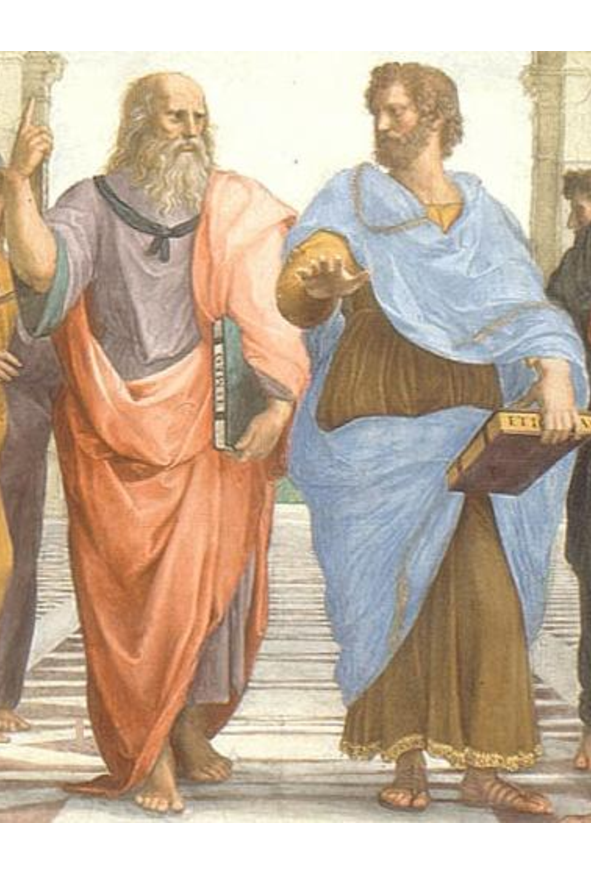
\includegraphics[width=4.5cm]{Plato_and_Aristotle_in_The_School_of_Athens,_by_italian_Rafael.pdf}
\caption{アテナイの学堂より:プラトンとアリストテレス}
\label{fig:Plato-Aristotle}
\end{wrapfigure}


これら「\textbf{それが何であるか?}」や「\textbf{それがどのようなものであるか?}」
といった問に対する回答についてより深く考察した人物がアリストテレスです.
 このアリストテレスとプラトンの思索の方向性の違いはラファエロ(Raffaello)
の有名な絵画「アテナイの学堂」\cite{アテナイ}にて中央に起立している両者の手の
違いで表現されていることはよく知られていることです. 図\ref{fig:Plato-Aristotle}
に示すようにプラトンは天上(イデア=抽象)を指し, アリストテレスは地上(形相=具象)
を示すという風にです. つまり, イデアは地上の個体から超越した存在であるのに対し,
 概念は個体の徴表から取り出されるものであるということです.
\newline

さて, そうして得られた概念は「\textbf{AはBである}」という命題であれば,
 複数の主語(A)の述語(B)となり得るという性質を持ちます. つまり, 概念はある
ものを語るものであり, だから対象Aを語るときに「AはXだ」となれば, まず概念
は対象Aの述語Xとして現れます. さらに対象Aだけに限定されずにほかの対象Bに
ついてもXであると言える可能性があるのです. この複数の主語に対して述語になる
性質を「\textbf{普遍}」と呼びます\footnote{いろいろなものを取り替えて使える
ものに「ユニバーサル」の名前を冠したものがあるのは, この主語を取り替えられる
性質に擬したためです.}. たとえば「\textbf{猫}」という「\textbf{概念}」は,
 その辺にいる「みけ」や「たま」, 周囲の野良猫 $x$ からでも
 「\textbf{$x$ は猫である}」という命題が作られます. だから「\textbf{猫}」と
いう「\textbf{概念}」は「\textbf{普遍}」なのです. その一方で「みけ」や
「たま」は個体に強く結びつけられて「これがたまです」という命題のように
個体を特定するものであって普遍ではありません. 
\newline

「猫」という括り(あつまり)に対しては「三毛猫」, 「黒猫」, 「白猫」,
 「虎猫」等の毛並で分類することができます. これらは「猫」の毛並について
述べたもので, こちらは「猫」という概念よりも個々の猫をより詳細に説明する
ものになっています. 逆に「猫」は「三毛猫」等を包括して説明しようとするもの
になっています. このように概念には「\textbf{類似する個体をまとめてより
包括的に説明しようとする概念}」, すなわち「\textbf{個体から離れた側の概念}」,
 それから逆に「\textbf{個体をより詳しく説明しようとする概念}」, 
 すなわち「\textbf{個体に近い側の概念}」の二つがあることが判ります. そして
「\textbf{対象を類似する対象とまとめて包括的に語ろうとする概念}」は
「\textbf{個体をより詳しく説明する概念}」を包含します. このように一つの
対象を語る二つの概念があって, 一方の概念が他方の概念を包含するときに包含
する側の概念のことを「\textbf{上位概念}」と呼び, 逆に個体をより詳しく
語ろうとする概念のことを「\textbf{下位概念}」と呼びます. これらの二つの
概念を比較すると上位概念が普遍になります. たとえば「三毛猫は猫である」
という命題では「猫」が上位概念, より細かく個体の「みけ」を説明している概念
が下位概念の「三毛猫」になります. 実際, 「三毛猫」は「猫である」と
「毛の色が黒・茶・白の三色である」の二つの性質が述べられるからです.
\newline

また上位概念を「\textbf{類概念}」, あるいは「\textbf{類(genus)}」,
 下位概念を「\textbf{種概念}」 あるいは「\textbf{種(species)}」と呼びます
\footnote{類と種の関係をここでは上位概念と下位概念として述べています
が, 「\textbf{種類}」という言葉があるように類(genus)と種(species)は
分類学では属(genus)と種(species)に対応し, 属の直下に種があってもその間
には何かが入ることはありません. このように種は類の直下にある概念としての
性格があります.}. 先程の「猫」で解説するならば「三毛猫の類概念」が「猫」,
「三毛猫」が「猫の種概念」になります. そして「\textbf{種}」の違いを示す
徴表(特徴)を「\textbf{種差}」と呼びます. たとえば先程の「三毛猫」, [虎猫」,
... の例では「毛並」の違いが種差になっています. それから「上位」,「下位」
はどちらが普遍であるかということに対応し, 普遍的な概念の外延は下位概念の
外延よりも広くなり, 上位概念は下位概念を包含し, このように概念の外延の
包含関係にも対応するのです. そしてには概念には上限と下限があり, 最上位の
概念を「\textbf{範疇(カテゴリー, Category)}」, 最下位の概念を
「\textbf{単独概念}」, あるいは「\textbf{個体概念}」と呼びます.
 この個体概念は個体を直接指示する概念で, 当然, 個体に最も近い概念です.
 それに対して範疇は個体を含む概念の中で最も普遍的な概念になります
\footnote{だからメニュー等では最上段が「\textbf{カテゴリー}」という
名称で分類されているのです.}.
\newline


この概念の階層構造についてはアリストテレスが「範疇(カテゴリー)論」等
の著作で述べています. ここでプラトンに批判的なアリストテレスのことを
イデア論が秘儀と化し始めた新プラトン主義の哲学者達からは「\textbf{師の
思想を秘匿するために批判していた}」と捉えられていたようで, 彼の論理学
は新プラトン主義の哲学への入門書としても重要視されます\footnote{当時の
ライバルのストア派の論理学は現代論理学に類似した命題論理学です. ただし
ストア派の論理学は断片でしか伝わっていません.}. アリストテレスの受容に
決定的だったのは, ポルピュリオス(\textgreek{Porf'urios}, Porphyry of
 Tyre)が記述した「\textbf{手引(エイサゴーゲー, \textgreek{E>isagwgh'},
 Isagoge\cite{Barnes}}」で, これがプラトンとアリストテレスを無理なく
結び付けることに成功し, 哲学を学ぶにあたって最初に読むべき本とされます.
 この「手引」によると「\textbf{ものごとを語る}」ということには
「\textbf{類}」, 「\textbf{種}」と「\textbf{種差}」に加えて
「\textbf{特有性}」と「\textbf{偶有性}」があると述べています. まず,
 類や種は「\textbf{それが何であるか?}」という問への回答です\footnote{
類(genus)と種(species)の語源はギリシャ語の\textgreek{g'enos}, 
 \textgreek{e\t{>i}dos}に由来し, 共に「\textbf{形}」という意味があり
ます. このことから概念は形の類似や違いをもとにしていた経緯が判るで
しょう. 分類学で当初はその形態, ダーウィン以降は進化, 現在はDNA等の
分析が入っています.}. それから「\textbf{種差}」と「\textbf{特有性}」と
「\textbf{偶有性}」は「\textbf{それがどのようなものであるか?}」という
問への答として語られるもので, 「\textbf{種差}」は
「\textbf{種を特徴付けるもの}」, それから「\textbf{特有性}」は
「\textbf{それが何であるかを語るものではないが指摘できるようなもの}」,
 つまり固有の特徴のことです. それに対して「\textbf{偶有性}」は
「\textbf{それの程度を語ることができるもの}」です. たとえば日焼けした子供
のように「全然日焼けていない」, 「薄く日焼けしている」, 
「良く日焼けしていて真っ黒」のように程度が表現可能で, そうでない状況
(「日焼けしていない」)」も考えられるのが特徴です. なお, このポルピュリオス
の「\textbf{類}」,「\textbf{種}」, 「\textbf{種差}」,「\textbf{特有性}」と
「\textbf{偶有性}」による述語の分類は非常に大きな影響をさまざまな分野に
与えています. たとえば「\textbf{ポルピュリオスの樹(Arbor Porphyrianae)}」
というものがあります:


\begin{itembox}[c]{\textbf{ポルピュリオスの樹}}
{\tiny
\begin{tikzpicture}
\Tree [.本質的存在 [.物体 [.生命がある [.理性的 [.人間 [.ソクラテス ]
                                                       [.プラトン ]
                                                       [.特定の人々 ] ] ]
                                       [.非理性的 ] ]
                          [.生命がない ] ]
                   [.非物体 ] ]
\end{tikzpicture}
}
\end{itembox}

これは類を下種で分類することをのちの註釈者が視覚化したもので, 様々な分野で
用いられています.
\newline

またリンネ(Carl von Linn\'e)が始めた動植物の学名の命名方法は
「\textbf{二名法}」と呼ばれますが, この方法は種による類の分類そのものです.
 つまりこの命名方法は動物/植物が属する種とその種を包含する属に対して最初に
属(genus)のラテン語名, それから種(species)のラテン語名を列記するものです
\footnote{正に「\textbf{種類}」になっているのです.}. たとえば人類の学名は
`Homo sapiens'で 属がHomoで種がsapiensです.
\newline

この二名法はオブジェクト指向プログラミングでも, クラスの属性やメソッド,
クラスとその直下のサブクラスの表記でも用いられています. このことからも判る
ように, オブジェクト指向プログラミングでは雛形としてクラスを準備することが
本質ではなく, 我々が対処しなければならない対象を語り, 明確に定義付けや特徴
付けといった分析を行うことこそが本質なのです.
\newline


さて「\textbf{それが何であるか?}」という問いに対し, 我々はそれがどのような
ものであるかを説明するか, そうでもなければ個体を列挙して説明するかのどちら
かになるでしょう. このように概念の表現には二通りの表現, 一つは
「\textbf{内包}」, もう一つが「\textbf{外延}」があります. 最初の
「\textbf{内包}」は概念が持つ徴表/属性で構成され,「\textbf{外延}」は概念が
適用される対象を列記することで構成されます. 「\textbf{猫}」という概念なら,
 その内包は「\textbf{動物である}」, 「\textbf{4本足で歩く}」,
 「\textbf{柔らかい肉球を持つ}」, 「\textbf{ニャオと鳴く}」等の属性から
構成されるでしょう. 一方で外延なら単純に「ペルシャ猫」, 「シャム猫」と
いった猫の種, 「黒猫」, 「白猫」, 「虎猫」, 「三毛猫」といった毛並で分類
する方法, あるいは「粟根さんのペットのタマ」のように個体を列記する方法に
なるでしょう. このように内包は概念を説明する述語から, 外延は概念に対応する
具体的な個体や下位概念の列記で構成されます.
\newline


そして内包と外延には「\textbf{内包外延反比例増減の法則}」と呼ばれる
関係があります. つまり, 内包が増大するに従って外延が減少し, 外延が増加すれ
ば内包が減少するという反比例関係です. たとえば「猫」という概念に対して
「茶、黒、白の三色の毛並である」という内包を追加すると「三毛猫」以外の
「白猫」, 「黒猫」等の猫が「猫」と「茶、黒、白の三色の毛並」の外延から消え
てしまいます. 逆に「三毛猫」という外延に「白猫」という外延を追加すると
「茶、黒、白の三色の毛並である」という内包が消えてしまいます. このように内包
が増えるということは, それだけ述語付けられることで個体に近付くために外延が
絞られ, 逆に外延を構成する個体が増えれば個体から離れて普遍的な事柄を抽出
することになるために内包が減少するということなのです.
\newline

なお外延で表現された概念は内包で説明規定することができますが, 逆に内包で
説明規定された概念は外延で表現できるとは限りません. さらに命題が必ず外延を
持つとは限りません. たとえば `$x \neq x$' という命題の外延は存在しません.
 この命題は発見者ラッセル(Russell)の名前を取って「\textbf{ラッセルの逆理}」
と呼ばれる逆理です. ラッセルがより分かり易くしたものが次に述べる
「\textbf{床屋の逆理}」です:

\begin{itembox}[c]{{床屋の逆理}}
\quad とある村には床屋が一軒だけあります. その床屋の主人は自分で髭を剃ら
ない人の髭だけを剃ると言っています. では, その床屋の主人の髭は誰が剃れば
よいでしょうか?
\end{itembox}


この逆理の破壊力は絶大でラッセルとフレーゲ(Frege)の論理主義\footnote{数学
を論理学から導出しようとする立場です. 初期はフレーゲの「算術の基本法則」
\cite{フレーゲ}, 後期はラッセルの「Principia Mathematica」\cite{Russell}
に代表され, その成果は現代数学の基礎の一つになっています.}は呆気なく破綻
してしまいます.
\newline


ポアンカレ(Poincar\'e)は「科学と方法」\cite{ポアンカレ}で逆理を分析し
ています(\cite{ポアンカレ},p.204). まず「偶数の集合」や
「身長170cm以下の人の集合」といった集合の定義は「自然数の集合」や
「人間の集合」といった根本の概念に触れずに定義ができており, このような
定義を「\textbf{可述的}」と呼びます. 一方で, 床屋の逆理のような循環論法
による定義を「\textbf{非可述的}と呼び, この非可述的な定義に問題があると
述べています. そこでラッセルは逆理を彼の体系から排除するために
「\textbf{型理論}」と「\textbf{悪循環原理}」を導入することで非可述的な
命題の排除に成功したものの, 今度は数学的帰納法が使えなくなるという副作用
が生じたため,  次に「\textbf{還元公理}」と呼ばれる公理を導入します. 
 ところが今度はその天下り的な性格が問題になるといった有様で, これらの
試みが成功したとは言えません\cite{Russell}. なお, 現在の集合論では公理系
で「\textbf{集合}」を定め, それ以外の命題の外延のことを「\textbf{類}」,
 あるいは「\textbf{クラス}」と呼んで集合と区分し, ラッセルの逆理を排除
しています.

\section{定義付けること}

さて我々は事物を抽象することで概念に辿りつきました. 逆に
「\textbf{Xを充すものがYである}」とも言える筈です. この操作を
「\textbf{定義付ける}」と言います. そして「\textbf{定義付ける}」ということに
「\textbf{タマは猫である}」 のように類や種で定義付ける「\textbf{実体的定義}」,
 あるいは 「\textbf{分析的定義}」と呼ばれる方法と
「\textbf{点は平面上の平行でない二直線の交わりとして構成される}」という点の
定義のように対象がどのような条件で発生, あるいは成立するかを記述する
「\textbf{発生的定義}」, または 「\textbf{綜合的定義}」と呼ばれる内包的な
定義があり, それと外延的な定義として
「\textbf{実例, または代表・典型を用いた定義}」があります.ちなみに
アリストテレスが創始者である逍遥学派の「\textbf{定義}」は類と種や種差を
用いてその「\textbf{説明規定}」を与えることです.


\section{プラトニズム}


では概念やイデアは実在するものでしょうか? イデア論を認めるのであれば,
 イデアは個体とは別に存在しますが, 概念の存在は厄介な問題です. たとえば
「三毛猫のみけ」を観察することで「猫」や「三毛猫」といった概念に到達できるとは
いえ, だからといって「みけ」が「猫」や「三毛猫」といった概念に先立って存在して
いる訳ではありません. それ以前に存在した猫や三毛猫によって「猫」や「三毛猫」
が定義されているからです. アリストテレスは範疇論で類や種を
「\textbf{第二の本質的な存在}」と呼んでいますが, それらが実際に存在するか
どうかを明確に述べていません. また前述のエイサゴーケでポルピュリオスが類や種
といった概念が存在するかどうかを触れないと最初の章で述べており, エイサゴーゲ
をラテン語に翻訳したボエティウス(Boethius)による第二注釈が西洋の
中世スコラ哲学での「\textbf{普遍論争}」を引き起すことになります\cite{普遍論争}.
\newline


ここで物理学の原理や数学の定理の方が先に存在して, それらを人間が発見すると考える
か, 到達した概念から原理や定理が導出されるものなのかといった議論にも,
 この議論は繋がります\footnote{「\textbf{発見}」なのか「\textbf{発明}」なのか?}.
 ここで事物の前に概念があると考える立場を「\textbf{プラトニズム(Platonism)}」,
 あるいはプラトンの「\textbf{実在論(Realism)}」と呼びます. それに対して事物の
あとに概念があると考える立場を「\textbf{唯名論(Nominalism}」と呼びます.
\newline


このように実在が問題となった背景ですが, アリストテレスが創始し, そこから発展
した伝統的論理学で扱う命題には「\textbf{存在含意(external import)}」と呼ばれ
る条件, つまり, 命題の主語が存在しているという暗黙の条件があります. これは
古代ギリシア語が属する印欧語族では `A = B' という命題の主語Aと述語Bの関係を
表現する「\textbf{繋辞(copula)}」に「\textbf{存在動詞}」が用いられていることが
関係しています. たとえば日本語の「AはBである」\footnote{「AはBで\underline{ある}」
という命題に「\textbf{ある}」が何気に含まれていることに, このような用語を作り定着
させた明治の人々の何気ない凄さを私は感じます.}を印欧語族の一つの英語に
「A is B」と置換したとき, 日本語の「は」はAとBが一致すること意味する以上の意味を
持ちませんが, be動詞は主語のAが存在するという意味が付随する存在動詞であるために
「Aが存在して A = B である」の意味を持つ命題として捉えることができるのです.
 ただし, 現代の論理学に存在含意はありません.
\newline 

また伝統的論理学は主語と述語の関係の考察を行なう「\textbf{名辞論理学}」
で, 現在の論理学は命題の真偽を基に考察する「\textbf{命題論理学}」です
\footnote{伝統的論理学に決定的に欠けているのが「\textbf{すべて}」や
「\textbf{存在する}」に対応する量化詞です.}. さて, 伝統的論理学の命題は,
 その主語に対して存在含意を前提にして論理学が構築されているために
「\textbf{非存在}」のものや「\textbf{仮説}」に対しては三段論法等の推論が
行えないことになります. しかし, ここでイデアや概念といった普遍の存在を
認めてしまえば, 自動的に存在含意を充して推論を行う際の障害がなくなるの
です. とはいえイデアにはその超越性から色々と面倒な問題が生じます.
\newline

最も有名なイデア論に対する反論が「\textbf{第三の人間}」と呼ばれるもので,
 まずイデア論者の主張するようにイデアの存在を認めると「\textbf{人間自体}」
という人間の類としてのイデアに加えて「\textbf{ソクラテス}」や
「\textbf{プラトン}」といった個人のイデアがあります. するとこれらのイデアで
人間として類似していることを示す尺度として, これらとはまた別の人間のイデアが
必要になります. これを「\textbf{第三の人間}」と呼びます. この第三の人間の存在
を認めると, 次はその「\textbf{第三の人間}」と個々の人間や人間自体のイデアとの
類似の尺度になる第四のイデアが必要になり, 以降, 第五, 第六...の人間が存在する
ことになるというものです.  この有様にプラトンの弟子であったアリストテレスも
「形而上学」\cite{アリストテレス2}にて「\textbf{物を数えようとする場合に,
 数が少なくては数えられないと思って, その数を増やして数えようとする者の
ごときである}」と批判しています\cite{アリストテレス2}
\footnote{形而上学 第一巻九章}.
\newline


また理想的な人間として例えられるソクラテスにしても, 赤ん坊, 子供, 若者,
 壮年, 老年といった過程を辿る訳ですが, すると, それぞれの瞬間にイデアが
ある筈で, その瞬間瞬間のイデア同士の関係はどうなるのかと話が簡単になる
どころか逆に複雑になっているありさまです. また種から芽が出てやがて木に
なり, それが老木になって倒れて腐るといった個体の生成, 変化や運動, 最後
に消滅する理由がイデア論からは説明できません. 結局, 機械仕掛けの神を
引っ張り出して創世神話や生物の生殖の理由を説明したとしても, 何気ない
現象の説明にはとても無理があるのです.


\section{形相(\textgreek{E\t{>i}dos})}

アリストテレスは師匠のプラトンと異なり, 観察に立脚したより現実に則した
考え方をしています. まず, 「\textbf{\textbf{形相(\textgreek{e\t{>i}dos},  
 eidos)}}」はプラトンの「\textbf{イデア(\textgreek{>idea})}」のような
「\textbf{個体から離れた存在}」(\textgreek{qorist'a})ではなく, むしろ, 現実
の個体を「\textbf{形相(\textgreek{e\t{>i}dos})}」と, これといった特性を
持たない「\textbf{質料(\textgreek{<'ulh})}」との「\textbf{結合体
(\textgreek{s'unolon}}」として捉え, この形相こそがその個体を個体
たらしめる原因, つまり「\textbf{形相因}」という設計図とプログラムのような
働きをするものとして捉えています. これを種の話に戻すと, まず, 種に木と
しての形相が内部に存在し, その形相が結合体としてのもう一方の質料に働き
かけることで木として育ち, やがて形相が木から消えることで木としての特性を
失って朽ちてゆくという説明になります. このアリストテレスの考察を現在の
科学と比べてどうかと言えば, 細かな点では怪しくとも, 現代の科学も研究対象
が何であり, どのような理由でそれがそれであるかを説明しようとするもので, 
 この流儀はアリストテレスの考察にその源流があることが判ります. だから
こそアリストテレスは「\textbf{万学の祖}」なのです.
\newline

この形相と質料の関係を計算機上で考えるとそれなりに面白いことが判ります.
 まず質料はそれ自体では何らの特性を持たないものですが, これをビットの列,
それから形相をデータ構造等の意味付けに対応付けることができるでしょう.
 すると計算機内部のデータは形相と質料の結合として表現されることになります.
 つまり, イデア論に訴えるよりもより自然な対応付けができるのです.


\section{アリストテレスの範疇(Category)}


個体が何であってどのようなものであるかを説明すること, すなわち,
 どのように述語付けられるかをアリストテレスは「範疇(カテゴリー)論」
\cite{アリストテレス1}にて説明しています. ここで範疇は最上位の概念で
あって最も普遍的なものであると述べましたが, この哲学用語の「\textbf{範疇}」
に対応するギリシャ語のカテゴーリアー(\textgreek{kathgori'a})は法律用語
の「\textbf{責を負わせる}」という意味のカテゴレイスタイ
(\textgreek{kathgor\~{i}estai})に由来し, アリストテレスが哲学用語として
導入した経緯があります. そして, この範疇はものことを語るときに, ものごと
に述語付けたり関連付けたりすること, すなわち, ものごとを述定することに
対応します.
\newline


アリストテレスは「範疇論」にて「\textbf{AはBである}」という命題の
述語Bが取り得るものを次の10個の範疇に分類しています:


\begin{itembox}[c]{{アリストテレスによる範疇}}
{\footnotesize
\begin{enumerate}
\item{まさにそれであるもの(本質的存在, 実体):「人間」,「猫」}
\item{どれだけか(量):「128cm」}
\item{どのようか(性質, 質):「面白い」, 「文法的」}
\item{何に対する(関係):「二倍」, 「半分」, 「より大きい」, 「より小さい」}
\item{どこか(場所):「千代田公園」,「ペットショップ」}
\item{何時か(時間):「昨日」, 「去年」}
\item{置かれている(態勢):「寝転んでいる」,「立っている」}
\item{持っている(所有):「靴を履いている」, 「首輪を付けている」}
\item{作用する(能動):「齧る」}
\item{作用を受ける(受動):「齧られる」}
\end{enumerate}
}
\end{itembox}


ここでの「\textbf{本質的存在(実体,\textgreek{o`us'ia})}」は
「\textbf{第二の本質的存在(第二実体)}」と呼ばれるものです. 第二があれば
第一もあり, その「\textbf{第一の本質的存在}」は「私」, 「みけ」,
「ソクラテス」等の個体で主語のみになるもの, つまり, 個体により近くて普遍性
を持たないものであるのに対し, 「\textbf{第二の本質的存在}」は「人間」,
 「猫」, 「哲学者」等の主語にも述語にもなり得るものです. そして, 類や種に
なり得るものでもあります. これらの本質的存在はギリシア語ではウーシアー
(\textgreek{o`us'ia})と呼ばれ, 英語のbe動詞に対応する「存在」を意味する
動詞\textgreek{e\~{'i}nai}を名詞化したものに由来するものです. この日本語
の訳語としては「\textbf{実体}」が当てられていますが, 本来のウーシアーの
意味する範囲は広いもので, ここでの訳語は範疇論\cite{アリストテレス1}の
新訳の用語に従っています.
\newline


なお, カント(Kant)は量, 質, 関係と様相の4綱目に分け, さらに
各自を3項目に分けて12の範疇にしています:


\begin{itembox}[c]{カントによる範疇の分類}
{\footnotesize
\begin{tabularx}{12cm}{X}
\begin{tabular}[t]{rl}
\ldelim\{{3}{30pt}[量 ]&
単一性\\
&数多性\\
&全体性\\
\end{tabular}
\\
\begin{tabular}[t]{rl}
\ldelim\{{3}{30pt}[質 ]&
実在性\\
&否定性\\
&制限性\\
\end{tabular}
%\right.
\\
\begin{tabular}[t]{rl}
\ldelim\{{3}{30pt}[関係]&
属性と実体性\\
&因果性(原因と結果)\\
&交互性\\
\end{tabular}
%\right.
\\
\begin{tabular}[t]{rl}
\ldelim\{{3}{30pt}[様相]&
可能性(不可能性)\\
&現実性(非現実性)\\
&必然性(偶然性)\\
\end{tabular}
%\right.
\\
\end{tabularx}
}
\end{itembox}


ここで重要なことは, ある物について「\textbf{それが何であるか?}」や
「\textbf{それがどのようなものであるか?}」という問に対する回答は,
 ここで述べた範疇の何れかになるということなのです. つまり, 我々が処理しよう
とする対象を記述するなら上記の範疇に収まり, そのようにして語られるものに
ついては, 類, 種, 種差, 特有性と偶有性によって階層構造が入るのです.
 そして, これらは我々が考察するオブジェクト指向プログラミングにおける
クラス表現に深く関わるのです.

\section{オブジェクト指向プログラミングにおけるクラスの表現}


ここでようやくオブジェクト指向プログラミングの話に戻しましょう. まず,
 扱うべき実際のデータが個体であり, このデータをオブジェクトが実体化したもの
として捉えられ, それから個体を何であるか, 何であるべきかを定める形相に相当
するものがオブジェクトのクラスに対応し, クラスの記述では, そのクラスを具体的
に定める属性を記載することになります. この属性はオブジェクトが
「\textbf{どのようなものなのか}」という問に対する回答が値で表現されればその
値,  何らかの機能であれば機能に対応するメソッドにすれば良いのです. たとえば
「猫」であれば「柔らかい肉球を持つ」, 「猫パンチで殴る」等の属性や機能が
あるでしょう. すると「猫」というクラスはこれらの猫の特徴(足の本数等々)を
列記し, 猫が持つ機能(「猫パンチ」,「雨の前に顔を洗うような仕草」等々)を
メソッドとして列記すればよいのです. そして, そのクラスで表現されたが
オブジェクトが「猫」であり, 「みけ」は「猫」というオブジェクトのインスタンス
として捉えられのです. このときにクラス間の関係はどのようになるでしょうか?
 ちなみに概念では類と種といった階層が入りますが, これに似たものとして次に
述べる「\textbf{継承}」という関係があります.


\section{継承}


概念にはより大きな外延を持つ上位概念と, より小さな外延を持つ下位概念
があります. 概念を内包で書換えてしまうと下位概念の内包は上位概念の内包を
基に, 上位概念に含まれない内包を付与したものになります. このことは上位概念に
含まれる属性をそのまま引き継いで, その概念に新しい属性を与えれば新たにその
下位概念が構築できることを意味します. この操作がオブジェクト指向
プログラミングでの「\textbf{継承}」に相当します.
\newline


この継承という考えは非常に自然な考え方です. 実際, ある新しい動物を発見
したときに, その動物の系譜が創られますが, その動物の調査が進むにつれて
さらに細かく分類されることもあります. この場合, 新しく分岐する動物は
もとの動物の分類を基にして新しい分類が行われるでしょう. これと同様に
扱うべきデータをとあるオブジェクトの実体化として記述したとしても, データ
への理解が深まることで, そのデータがより細かく分類されることはそう珍しい
ことではありません. このことは最初に大きく分類したクラスを, より下位の
クラスへとさらに細かく分割することに相当しますが, この細分化は上位の
クラスにない値やメソッドを追加することで行われます. そして, この処理
は最初のクラス構築が間違っていない限り, システムの大枠を変更すること
なしに自然に拡張が行えることを意味するのです.
\newline


この継承を手際よく行うためには的確な分析が必要であることは言うまでも
ありませんが, この的確さには経済的な側面もあります. 実際, 継承関係が
一子相伝的な継承であれば継承は直線的な関係になるので属性やメソッドが
どこから引き継がれたかを探すことが容易ですが, 実際の継承は複数のクラス
からの継承を含む複雑なものになるでしょう. ここで複雑怪異, あるいはやたら
詳細な親子関係になっていれば, 扱う側にとっても不要な混乱を招くだけで
はなく, メソッドや属性の検索という利用上の観点からも不利になるのです.
 実際, クラスを分類を細かくしてしまえばどうなるでしょうか?  たとえば
「猫」から個体の「みけ」に至るまでに「三毛猫」が間に一つ入る場合と
「アジアの猫」,「東アジアの猫」,「日本猫」,「三毛猫」が入る場合を比較
すると, 猫の毛並の話だけなら「アジア」, 「東アジア」, 「日本」は不要
です. さらに「みけ」が持つ「猫の属性」や「猫の習性」を知りたくなると,
 最初に「みけ」が属するクラスから順に調べることになりますが, 前者の
継承関係なら「三毛猫」を間に一つ挟む程度で済むことが, 後者の継承関係
では「アジアの猫」, 「東アジアの猫」と「日本猫」の三つのクラスで検索を
行う必要が出てくるのです. このように複数のクラスの継承では属性やメソッド
の検索により多くの時間を要することになり, おまけに属性やメソッドの
検索順位をどのように定めるかで新しいクラスの属性やメソッドが反映されなく
なる問題も生じます. この問題については「\textbf{C3 MRO}」といった手法で
改善が図られていますが, 最初のクラスの分析が非常に重要であることは
言うまでもないことです.

\section{おわりに}

最後にニーチェの「悲劇の誕生」\cite{悲劇の誕生}の末尾の言葉で締め括りたいと
思います. 「...奇妙な異国の人よ, しかし, またこうも言っていただきたい.
 この民族がこれほど美しくなるためには, どんなに悩まなければならなかった
ことか!と...」. そう, 「\textbf{みーんな悩んで大きくなったぁ!!}」\cite{野坂}
\footnote{ここでにやにやしている貴方は間違いもなくオジサン, オバサンです.}
のです!

\begin{thebibliography}{99}
\bibitem{アリストテレス1}
アリストテレス, アリストテレス全集1 カテゴリー論・命題論, 岩波書店,2013.
\bibitem{アリストテレス2}
アリストテレス, 形而上学(上下), 岩波文庫.
\bibitem{トピカ}
アリストテレス, (旧)アリストテレス全集2, トピカ・詭弁論駁論, 岩波書店, 1987.
\bibitem{ゲーテ}
ゲーテ(著), 相良守峯(訳), ファウスト(第一部,第二部),岩波文庫, 岩波書店,1958.
\bibitem{クラウス}
クラウス(著), 池内紀(訳), 
カール・クラウス著作集 9・10 人類最期の日々, 法政大学出版局, 2001.
\bibitem{クラーザー}
クラーザー(著), 関楠生(訳), ドイツ第三帝国, 中公文庫, 中央公論新社, 2008.
\bibitem{柴田}
柴田有,グノーシスと古代宇宙論,勁草書房,1982.
\bibitem{関}
関楠生(編訳),ヒトラー・ジョーク, 河出書房新社, 1983.
\bibitem{藤野}
藤野登, 論理学 -伝統的形式論理学-,内田老鶴圃, 2003.
\bibitem{国家}
プラトン(著), 藤沢 令夫(訳), 国家, 岩波文庫, 岩波書店, 1976.
\bibitem{フレーゲ}
フレーゲ,フレーゲ著作集3 算術の基本法則,勁草書房,2000.
\bibitem{ポアンカレ}
ポアンカレ(著),吉田洋一(訳),科学と方法,岩波文庫,岩波書店,1953. 
\bibitem{墨子}
薮内清,墨子, 東洋文庫,平凡社,1996.
\bibitem{悲劇の誕生}
ニーチェ(著), 秋山英夫(訳), 悲劇の誕生, 岩波文庫, 岩波書店, 1966.1
\bibitem{ツァラトゥストラ}
ニーチェ(著), 水上英廣(訳), ツァラトゥストラはこう言った(上下), 
岩波文庫, 岩波書店, 1970.
\bibitem{普遍論争}
山内志朗, 普遍論争, 平凡社ライブラリー, 2008
\bibitem{錬金術}
吉田光邦, 錬金術 - 仙術と科学の間 -, 中央公論新社, 2014.
\bibitem{Barnes}
J.Barnes, PORPHYRY INTRODUCTION,Oxford University Press, 2006.
\bibitem{Russell}
B.Russell \& A.N.Whitehead,Principia Mathematica to *56,
Cambridge Mathematical Library,Cambridge University Press,1997.
\bibitem{アテナイ}
アテナイの学堂 
http://ja.wikipedia.org/wiki/アテナイの学堂
\bibitem{野坂}
野坂昭如
https://www.youtube.com/watch?v=A-89Rv3yZ44
\end{thebibliography}



\end{document}
\end
\end








